%!TEX root = ../../main.tex

Para a AlexNet, assim como para a CNN anterior, foi realizada uma busca em \emph{grid} para ambas as abordagens, utilizando os hiperparâmetros selecionados anteriormente, gerando assim, mais $72$ modelos a serem avaliados quanto às suas métricas de desempenho.

Considerando a métrica de \emph{F-Score}, foram selecionados os melhores modelos  desta arquitetura e estes encontram-se listados na Tabela \ref{tab:alexnet}. Na Figura \ref{fig:treinamento-alexnet} pode-se observar os gráficos com os comportamentos dos valores de \emph{loss} e acurácia encontrados nos conjuntos de treinamento e validação durante o estágio de treino destes modelos.

\begin{table}[h!]
\centering
\caption{Detalhamento dos melhores modelos obtidos com a arquitetura AlexNet para cada uma das abordagens consideradas neste trabalho.}
\label{tab:alexnet}
\resizebox{\textwidth}{!}{\begin{tabular}{ccccccc}
\toprule
\textbf{Abordagem} & \textbf{Otimizador} & \textbf{\emph{Patience}}  & \textbf{Função de Ativação} & \textbf{Acurácia} & \textbf{F-Score} & \textbf{EER} \\
\midrule
Abordagem A & Adam & 15 & ELU & $0.9654$ & $0.9393$ & \\
Abordagem B & RMSprop & 5 & ELU & $0.8593$ & $0.7993$ & $13.8265$\\
\bottomrule
\end{tabular}}
\end{table}

\begin{figure}[H]
 \centering
 \caption{Histórico de \emph{loss} e acurácia durante o treinamento dos melhores modelos obtidos com a arquitetura AlexNet.}
 \label{fig:treinamento-alexnet}
 \subfloat[\emph{Loss} durante treinamento da melhor rede AlexNet para a abordagem A.\label{subfig:alexnet-a-loss}]{%
 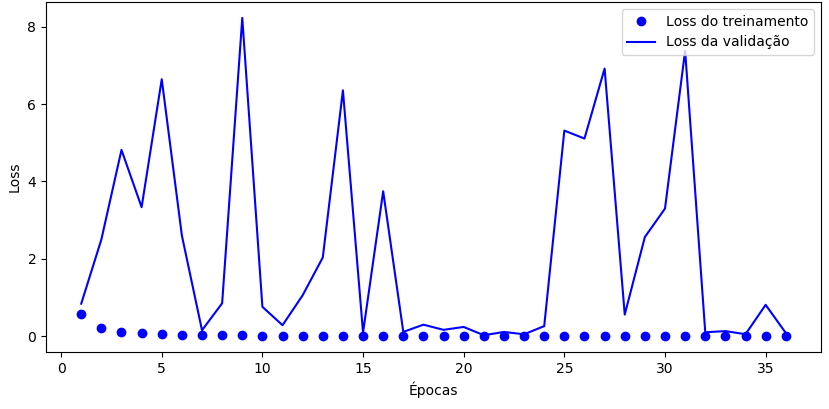
\includegraphics[width=0.47\textwidth]{imgs/alexnet-a-loss}
 }
 \hfill
 \subfloat[Acurácia durante treinamento da melhor rede AlexNet para a abordagem A.\label{subfig:alexnet-a-acc}]{%
 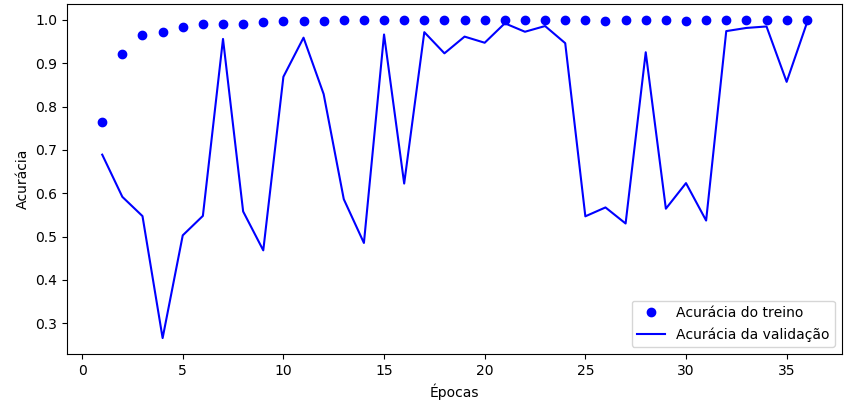
\includegraphics[width=0.47\textwidth]{imgs/alexnet-a-acc}
 }
 \hfill
 \subfloat[\emph{Loss} durante treinamento da melhor rede AlexNet para a abordagem B.\label{subfig:alexnet-b-loss}]{%
 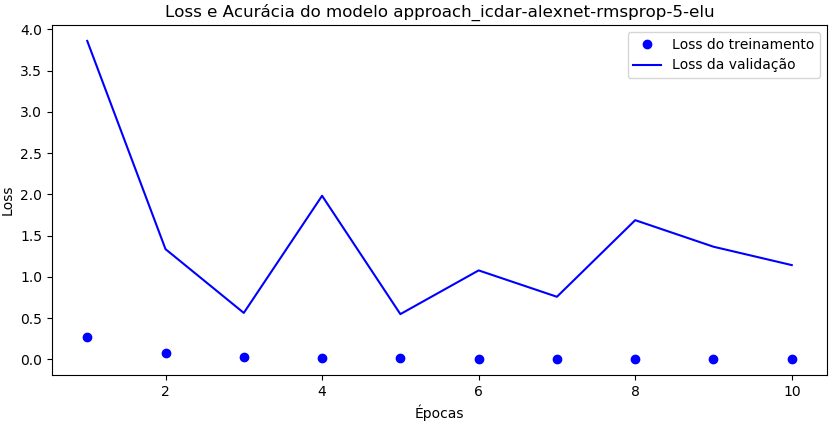
\includegraphics[width=0.47\textwidth]{imgs/alexnet-b-loss}
 }
 \hfill
 \subfloat[Acurácia durante treinamento da melhor rede AlexNet para a abordagem B.\label{subfig:alexnet-b-acc}]{%
 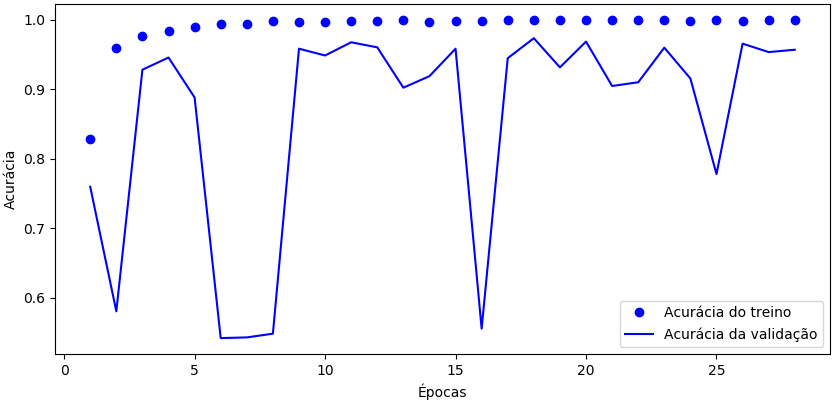
\includegraphics[width=0.47\textwidth]{imgs/alexnet-b-acc}
 }
\end{figure}

Considerando que estas redes possuem mais parâmetros treináveis, este possivelmente foi um fator responsável pelo maior números de épocas no treinamento na abordagem A. Nota-se ainda que houve oscilações nos treinamentos, resultando em parada precoce. Para esta arquitetura, as redes treinadas com a função de ativação ELU mostraram métricas melhores na etapa de avaliação.

Observando as métricas de acurácia e \emph{F-Score} obtidas, percebe-se que estas foram inferiores às observadas para as redes LeNet, mas ainda assim alcançando valores superiores a $90\%$ na abordagem A e valores próximos a $80\%$ na abordagem B. 

Examinando mais atentamente o desempenho destas redes no conjunto de testes, tem-se as matrizes de confusão mostradas na Figura \ref{fig:matrizes-alexnet}.No melhor modelo da abordagem B, para esta arquitetura, a disposição dos valores na matriz de confusão mostra uma reflexão diferente da encontrada no cenário LeNet. Neste caso, houve uma quantidade maior de falsos positivos, mostrando a dificuldade na detecção das assinaturas \emph{over-the-shoulder} realizadas pelos autores forjadores.

\begin{figure}[H]
 \centering
 \caption{Matrizes de confusão dos melhores modelos obtidos com a arquitetura AlexNet.}
 \subfloat[Melhor AlexNet para a abordagem A\label{subfig:matriz-alexnet-a}]{%
 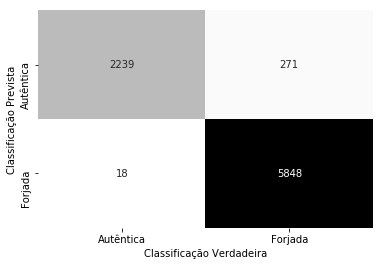
\includegraphics[width=0.47\textwidth]{imgs/matriz-alexnet-a}
 }
 \hfill
 \subfloat[Melhor AlexNet para abordagem B\label{subfig:matriz-alexnet-b}]{%
 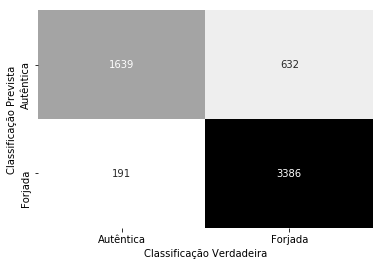
\includegraphics[width=0.47\textwidth]{imgs/matriz-alexnet-b}
 }
 \label{fig:matrizes-alexnet}
\end{figure}

De modo geral, apesar de possuir boas métricas, o melhor modelo encontrado pela arquitetura AlexNet, com um \emph{F-score} de $0.9393$, não foi suficiente para superar o melhor modelo obtido com a arquitetura LeNet ($0.9755$). Uma vez que a arquitetura LeNet possui menos parâmetros que a AlexNet e melhor desempenho observado, ressalta-se a sua maior adequação para a tarefa considerada, acrescido ao fato de demandar menos recursos de tempo de treinamento e de memória para seu armazenamento.
